\documentclass[tikz,border=8pt]{standalone}
\usepackage{fontspec}
\setsansfont{Arial}
\usetikzlibrary{arrows.meta,positioning,fit}
% Proposed SDP II pipeline for the dismantled project (Section 4.6). Nothing in this
% diagram is implemented except the shared scan-result contract.
\begin{document}
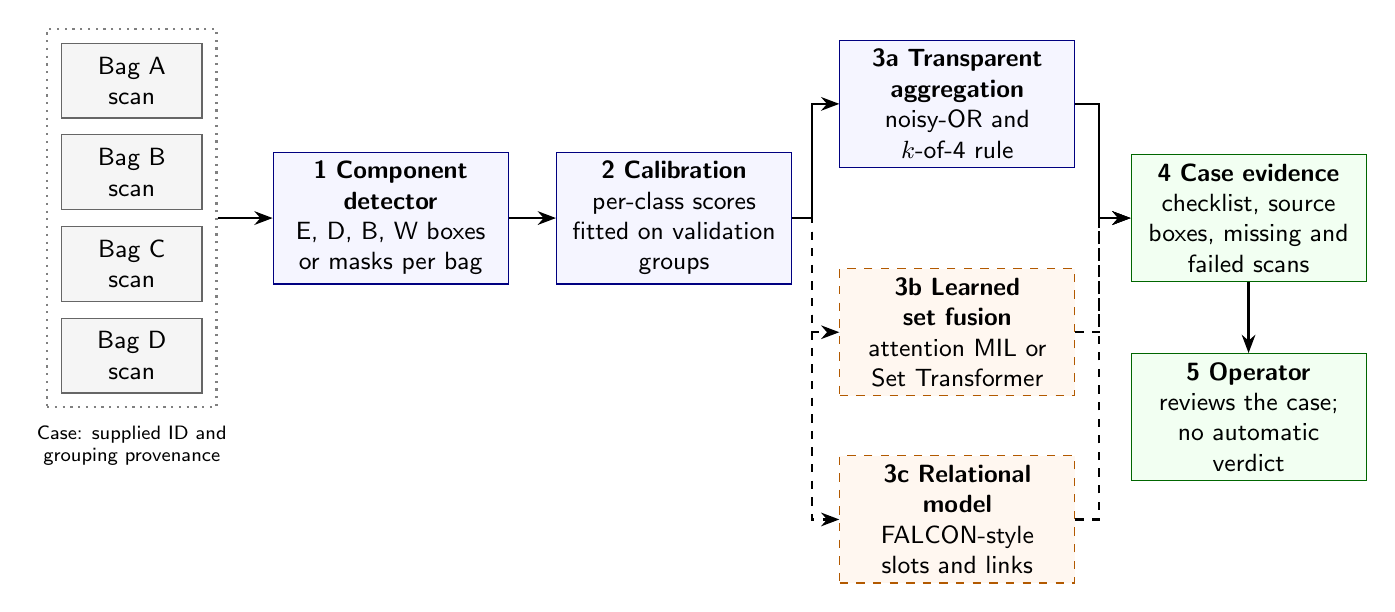
\begin{tikzpicture}[font=\sffamily\small,>=Stealth,
bag/.style={draw=black!60,align=center,text width=1.55cm,minimum height=0.95cm,fill=black!4},
box/.style={draw=blue!50!black,align=center,text width=2.75cm,minimum height=1.5cm,fill=blue!4},
opt/.style={draw=orange!70!black,dashed,align=center,text width=2.75cm,minimum height=1.5cm,fill=orange!6},
fin/.style={draw=green!40!black,align=center,text width=2.75cm,minimum height=1.5cm,fill=green!5}]
\node[bag] (a) {Bag A\\scan};
\node[bag,below=0.2cm of a] (b) {Bag B\\scan};
\node[bag,below=0.2cm of b] (c) {Bag C\\scan};
\node[bag,below=0.2cm of c] (d) {Bag D\\scan};
\node[draw=black!50,dotted,thick,fit=(a)(b)(c)(d),inner sep=5pt] (case) {};
\node[below=0.1cm of case,align=center,font=\sffamily\scriptsize] {Case: supplied ID and\\grouping provenance};
\node[box,right=0.7cm of case] (det) {\textbf{1 Component\\detector}\\E, D, B, W boxes\\or masks per bag};
\node[box,right=0.6cm of det] (cal) {\textbf{2 Calibration}\\per-class scores\\fitted on validation\\groups};
\node[box,right=0.6cm of cal,yshift=1.45cm] (agg) {\textbf{3a Transparent\\aggregation}\\noisy-OR and\\$k$-of-4 rule};
\node[opt,right=0.6cm of cal,yshift=-1.45cm] (set) {\textbf{3b Learned\\set fusion}\\attention MIL or\\Set Transformer};
\node[opt,below=0.75cm of set] (rel) {\textbf{3c Relational\\model}\\\mbox{FALCON-style}\\slots and links};
\node[fin,right=0.7cm of agg,yshift=-1.45cm] (res) {\textbf{4 Case evidence}\\checklist, source\\boxes, missing and\\failed scans};
\node[fin,below=0.9cm of res] (op) {\textbf{5 Operator}\\reviews the case;\\no automatic\\verdict};
\draw[->,thick] (case)--(det);\draw[->,thick] (det)--(cal);
\draw[->,thick] (cal.east)--++(0.25,0)|-(agg.west);
\draw[->,thick,dashed] (cal.east)--++(0.25,0)|-(set.west);
\draw[->,thick,dashed] (cal.east)--++(0.25,0)|-(rel.west);
\draw[->,thick] (agg.east)--++(0.3,0)|-(res.west);
\draw[->,thick,dashed] (set.east)--++(0.3,0)|-(res.west);
\draw[->,thick,dashed] (rel.east)--++(0.3,0)|-(res.west);
\draw[->,thick] (res)--(op);
\end{tikzpicture}
\end{document}
